
\subsection{L'achat d'un architecte}
\label{canbuy}

\subsubsection{Algorithme glouton}

L'algorithme glouton va chercher si on est capable de payer le prix et renvoyer la première façon de le faire.

Pour cela on retire au prix à payer la production de tous les architectes, puis va parcourir l'ensemble des jetons du joueur. Dès qu'un jeton peut être utilisé pour payer le prix, on retire au prix ce que procure le jeton et on l'ajoute au marché utilisé pour payer (qui est retourné à l'issu de l'algorithme).

\begin{lstlisting}[language=pascal, frame=single, caption={Algorithme glouton de rendu de monnaie}]
procedure rendu_glouton(var guilde : Guilde; var ressources : Marche; prix : Set);
var
    i: integer;
    jeton : Jeton;
    out : Marche;
begin
    for i := 0 to MAX_BUILDER do
    begin
        prix := retirer_au_prix(prix, builder[i].provide)
    end;

    for i := 0 to NUM_TOKENS do
    begin
        jeton := ressources[i]
        if utilisable(prix, jeton) then
        begin
            ajouterJeton(out, jeton);
        end;
        if prix == set_nul then
        begin
            retourner out;
        end;
    end;

    return set_nul;
end;

\end{lstlisting}

La complexité de cet algorithme est linéaire par rapport au nombre maximum de jetons. 

\subsubsection{Algorithme récursif}

Contrairement à un algorithme glouton, l'algorithme récursif va permettre de récupérer la meilleur façon de payer un architecte. 

Tout comme l'algorithme glouton, on commence à retirer au prix ce qui est produit par les architectes. On teste ensuite l'ensemble des combinaisons de jetons (stocké dans un marché) pour payer le prix.

A chaque fois que l'on peut utiliser une combinaison pour payer le prix, on compare cette combinaison avec la précédente pour sélectionner la meilleure (cf \ref{market_cmp}). On teste l'ensemble des des combinaisons de nb-jetons avec nb variant entre 1 et le nombre de ressrouces dans le prix à payer.

Avec les k-uplets suivants représentant l'ensemble des jetons présents dans le marché testé, l'arbre des appels du rendu de monnaie est construit comme suivant :

\begin{figure}[H]
    \centering
    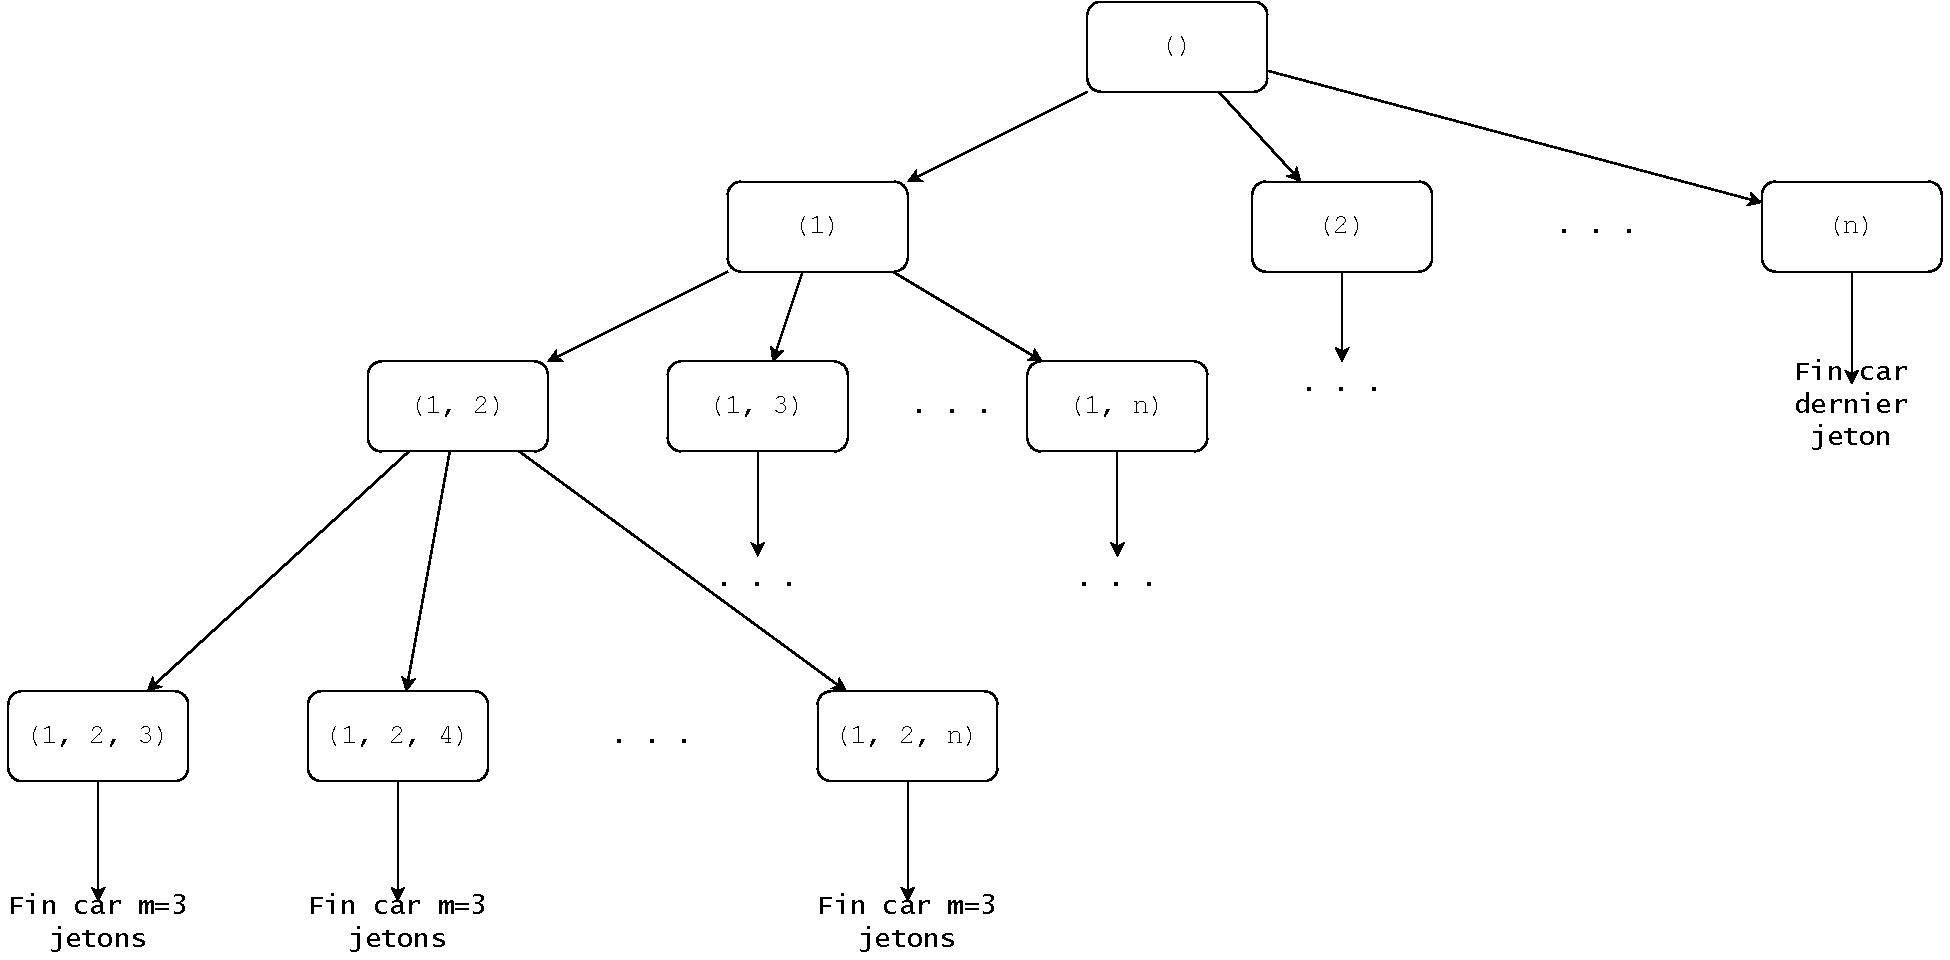
\includegraphics[width=\textwidth]{img/call_tree.pdf}
    \caption{Arbre des appels du rendu de monnaie}
    \label{fig:enter-label}
\end{figure}

L'algorithme pour tester les combinaisons de nb-jetons ressemble à cela :

\begin{lstlisting}[language=C, frame=single, caption={Algorithme de test des combinaison de nb-jetons}]
void find_max_eff_sub_market_rec(args)
{
    if (est_utilisable(marche_teste))
        if (non est_utilisable(meilleur))
            meilleur = marche_teste;
            
        else
            *meilleur_marche = max_marche(meilleur_marche, marche_teste);

    else if (k < m)
    {
        for (chaque appel du dernier indice a n)
            /* Appel recursif */;
    }
}
\end{lstlisting}

\subsubsection*{Complexité, terminaison et correction}
\subsubsection*{Complexité}
L'algorithme de rendu de monnaie teste l'ensemble des combinaisons de jetons. 

Or :

\begin{equation}
    \sum_{k=1}^{n} \binom{n}{k} = 2^n
\end{equation}

avec n le nombre de jetons maximum pour un joueur. Tester si un marché est utilisable se fait en complexité linéaire.

On a donc une complexité exponentielle en $\Theta(n2^n)$.
\begin{summary}
Cependant le prix maximum ne possède jamais autant de couleur que le nombre de jeton que possède un joueur. Dans notre cas de figure, le prix se limite à $m = 3$ couleurs différentes.

Ainsi on ne va tester seulement $\displaystyle \sum_{k=1}^{m} \binom{n}{k}$ combinaisons de jetons. La complexité de l'algorithme est donc grandement diminué et on a plutôt un algorithme en $O(n^m)$ lorsque $m$ ne dépend pas de $n$, ce qui est le cas dans notre version actuelle du jeu.
\end{summary}

\subsubsection*{Terminaison}

À chaque appel récursif, $k$ augmente de $1$, donc en considérant $m = resources\_requises$, on peut poser un variant $V = m - k$, qui un entier naturel strictement décroissant.

On a donc la terminaison du rendu de monnaie.

\subsubsection*{Correction}

On note :

\begin{itemize}
    \item a\_acheter est l'ensemble de ressource qu'on essaie d'acheter
    \item eff(marché): float une fonction qui associe à un marché une efficacité, le but est de la maximiser
    \item est\_utilisable(marché): booléen retourne vrai si marché permet de payer a\_acheter
    \item "meilleur" le meilleur marché jusqu'à présent au sens de eff
    \item max\_marche(marché1, marché2): marché retourne le meilleur marché entre marché1 et marché2 au sens de eff
\end{itemize}
 

On pose :

\begin{itemize}
    \item PRECOND = "non est\_utilisable(\code{meilleur}) $\Rightarrow$ \code{meilleur} = $\emptyset$"
    
    \item POSTCOND = "si est\_utilisable(\code{meilleur}) alors eff(\code{meilleur}) = max(efficacité des sous-marchés utilisables, sinon meilleur = $\emptyset$"
\end{itemize}


\subsubsection*{Démonstration par induction}

\noindent Si PRECOND,

\textbf{Cas de base :}

Si est\_utilisable(\code{marché\_test}), alors 

\begin{itemize}
    \item Si eff(\code{marché\_test}) > eff(\code{meilleur}), alors \code{meilleur} $\leftarrow$ \code{marché\_test}

    \item sinon, on a bien que \code{meilleur} est plus efficace que \code{marché\_test}
\end{itemize}

Sinon, si $num\_token(marche\_test) > m$, alors on ne fait pas d'appels récursifs, et étant donné que les appels nous ont menés jusqu'au marché \code{marché\_test}, cela veut dire que les marchés précédents ne permettent pas d'acheter \code{a\_acheter}, et donc \code{meilleur} est toujours maximum.

\textbf{Induction :}

Notre appel récursif se fait sous cette forme :

\begin{lstlisting}[language=C, frame=single, caption={Appels récursifs du rendu de monnaie}]
pour (indice de prochain_indice a n)
{
    nouveau_marche = cree_prochain_marche(marche_test, indice)

    appel_recursif(nouveau_marche)
}
\end{lstlisting}

On a clairement la terminaison de la boucle pour.

On pose l'invariant I comme suivant :

"si est\_utilisable(meilleur), alors $\forall i \in \{prochain, ..., k\}, \forall $ marché découlant de $nouveau\_marche_i$, $eff(meilleur) \geq eff(nouveau\_marche_i)$. Sinon, $meilleur = \emptyset$"

\textbf{Première itération}

Au début de l'itération, d'après PRECOND, si non est\_utilisable(meilleur), Alors $meilleur = \emptyset$.

Sinon, $k = 0$, donc on a bien l'inégalité de I.

Finalement, I est vraie à l'initialisation.

\textbf{Récurrence}

Soit $k$ un entier entre $prochain$ et $n$, on suppose que notre invariant est vrai pour l'itération $k$.

Sachant qu'on a supposé que POSTCOND de l'appel récursif sur $nouveau\_marche_k$ est vrai, on obtient que $\forall  marche$ découlant de $nouveau\_marche_{k + 1}$, $eff(meilleur) \geq eff(marche)$.

Or, par hypothèse de récurrence, on avait que meilleur était déjà le maximum des marchés découlant des $k$ premiers nouveau\_marchés, il est donc maintenant le meilleur des marchés découlant des $k + 1$ nouveaux\_marchés.

On a donc par récurrence :
"si est\_utilisable(meilleur), alors $\forall i \in \{prochain, ..., n\}, \forall $ marché découlant de $nouveau\_marche_i$, $eff(meilleur) \geq eff(nouveau\_marche_i)$. Sinon, $meilleur = \emptyset$"

Ce qui est équivalent à POSTCOND, et qui montre la correction de l'algorithme.
